\DeclareSong{If You Come Back To Haunt Me}{Radical Face}{Once A Hue, Always A Hue}[4]
\intro{D\pause G\rep{8}}
\begin{strophe*}
  \begin{tabular}{l l}
   You might \chord[c]{D}come, &
   And you might \chord[c]{G}break me \tbnl

   But I know my \chord[c]{D}place, &
   'cause I was born \chord[c]{G}into it \tbnl

   And you might \chord[c]{D}crash, &
   And you might \chord[c]{G}burn up \tbnl

   But you know your \chord[c]{D}place, &
   'cause you dug yourself \chord[c]{G}into it \tbnl

   And they might \chord[c]{D}win, &
   And they might \chord[c]{G}break me \tbnl

   But I know my \chord[c]{D}place, &
   'cause I'm getting \chord[c]{G}used to it \tbnl

   And you might \chord[c]{D}live, &
   Or you might \chord[c]{G}give up \tbnl

   But you know your \chord[c]{D}place,\Pause\null &
   'cause you've fallen \chord[c]{G}into it \tbnl

   And I'm falling \chord[c]{D}too
  \end{tabular}
\end{strophe*}
\interlude{D\pause G\rep{4}\Pause D\pause A\pause G\pause Bm\pause A\pause G\pause A\pause\rep{3}}
\begin{chorus*}
  And if \chord[c]{D}you come \chord[c]{A}back to \chord[c]{G}haunt me

  I could \chord[c]{Bm}probably \chord[c]{A}use the \chord[c]{G}company

  Come \chord[c]{A}have a seat

  But \chord[c]{D}I have be\chord[c]{A}come for\chord[c]{G}getful

  I can't re\chord[c]{Bm}member \chord[c]{A}why you \chord[c]{G}died

  And \chord[c]{A}how \chord[c]{Bm}all this \chord[c]{A}feels like a \chord[c]{G}daydream

  Or \chord[c]{A}like some \chord[c]{D}ghostly \chord[c]{A}play

  Where \chord[c]{Bm}every\chord[c]{A}thing that is \chord[c]{G}happening

  \chord[c]{A}Looks \chord[c]{D}like it's \chord[c]{A}dead and \chord[c]{D}gone
\end{chorus*}
\interlude{D\pause G\rep{4}}
\begin{strophe*}
  \begin{tabular}{l l}
   And I won't \chord[c]{D}bend, &
   So you'll have to \chord[c]{G}break me \tbnl

   But I know my \chord[c]{D}place, &
   And I'm pretty \chord[c]{G}used to it \tbnl

   And you might \chord[c]{D}turn, &
   And you might lose \chord[c]{G}face, \tbnl

   But you know your \chord[c]{D}place, &
   'cause you've given \chord[c]{G}into it \tbnl

   And you might \chord[c]{D}love, &
   Or you might \chord[c]{G}hate me, \tbnl

   But I know my \chord[c]{D}name, &
   And I'm pretty \chord[c]{G}used to it \tbnl

   And you might \chord[c]{D}turn, &
   And you might \chord[c]{G}leave me \tbnl

   But I know my \chord[c]{D}place, &
   And I've gotten \chord[c]{G}used to it \tbnl
  \end{tabular}
\end{strophe*}

\outro{\rep{5, ad infinitum}}\vskip -0.7em
\begin{strophe*}
  And I've gotten \chord[c]{D}used to it\dots \PAUSE And I've gotten \chord[c]{G}used to it\dots
\end{strophe*}

\vfill
\begin{center}
 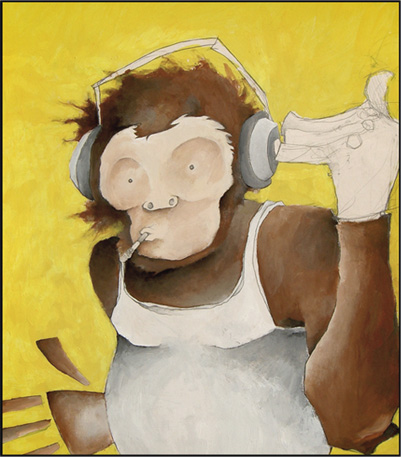
\includegraphics[scale=3]{pni9.jpg}
\end{center}
\vfill